\documentclass[]{article}

\usepackage{float}
\usepackage{graphicx}
\usepackage[export]{adjustbox}

%opening
\title{Parallel System Architectures --- Lab 3}
\author{Andrea Di Dio --- 12967424}

\begin{document}

\maketitle

\section{Design Choices}

For this assignment, the cache model differs once again from the previous assignment because it changes to a write-back model. The lab required to implement the MOESI protocol for cache coherence and this section will give a high level explanation of how this was implemented in the code.\\
The first change applied from the second lab is that there is an extra signal (\textit{port\_c2c\_*}) connecting the bus and the caches in order for the caches to let the bus know that a certain word does not have to be fetched from main memory but can be satisfied by another cache. Whenever a new bus request is placed in the queue, the bus writes to the c2c port such that caches snooping the bus, if they have ownership of the data, can check if they can satisfy the request. If they do, they call the \textit{cache\_to\_cache()} method, which replaces the request in the queue with a request holding the \textit{is\_c2c} variable to \textit{true}. The requests in the queue which hold this property are prioritized by the arbiter for fast completion of the request.\\
The second change made is a direct consequence of the change in the cache model to a write-back scheme. Whenever a line is evicted due to being the LRU line, if the line to be evicted is either in the modified or owned state, it must be written back to main memory in order to maintain consistency of data. Changing to a write-back cache model also results in not writing through on a cache write. Instead, a write will result in a cache line becoming valid and going to the modified state.\\
Lastly, in the second assignments were only snooping for other processor writes to invalidate their own cache line. For this assignment, caches snoop for both reads and writes from the other caches. On a probe write, cache lines are still invalidated, whilst on a probe read, cache lines with the exclusive bit set move to the shared state, and those with the modified bit set move to the owned state.\\
One issue with MOESI caches is that whenever a CPU tries to read or write to a location for which the data is held by another cache and the data is not yet written back to main memory, it might get a non-consistent version of the data. There are two possible workarounds to this problem, one being that we force a writeback from the other processor holding the up-to-date copy, the other being that we implement a cache-to-cache transfer for that data. I decided to implement the latter method in order to avoid the latency of having two extra operations to main memory (the first write for the writeback operation and the read from the processor which originally requested the data). This is implemented in the \textit{Cache::snoop()} thread similarly to other cache-to-cache transfers.

\section{Results}

This section will report the results for the experiments with the tracefiles as in other labs. Due to the fact that even a cache-to-cache transfer is registered as a read or write miss for the requesting processor, I expect the hitrates for this cache model to be very similar to those from the previous lab. On the other hand, i expect the number of memory operations (reads and writes) to be significantly lower for the MOESI cache coherence protocol due to the number of cache-to-cache transfers which were not possible in the VALID-INVALID protocol and also because the cache model is write-back and not write-through, meaning that modifying the data won't cause additional writes to main memory. This section will also present the results of turning off snooping for the caches and compare the amount of memory reads and writes with the normal (with snooping) protocol.


\subsection{Debug Tracefile}

\subsubsection{2 processors}

\begin{table}[H]
	\begin{tabular}{|l|l|l|l|l|l|l|l|}
		\hline
		\textbf{CPU} & \textbf{Reads} & \textbf{RHit} & \textbf{RMiss} & \textbf{Writes} & \textbf{WHit} & \textbf{WMiss} & \textbf{Hitrate} \\ \hline
		0            & 30             & 0             & 30             & 25              & 1             & 24             & 1.818182         \\ \hline
		1            & 32             & 0             & 32             & 35              & 1             & 34             & 1.492537         \\ \hline
	\end{tabular}
\end{table}

Total Memory Reads = 65 Total memory Writes = 2 (Total = 67)\\
Average Bus Acquisition Time = 1690176 ps\\
Total Simulation Time = 6769 ns 

\subsubsection{4 processors}

\begin{table}[H]
	\begin{tabular}{|l|l|l|l|l|l|l|l|}
		\hline
		\textbf{CPU} & \textbf{Reads} & \textbf{RHit} & \textbf{RMiss} & \textbf{Writes} & \textbf{WHit} & \textbf{WMiss} & \textbf{Hitrate} \\ \hline
		0            & 8              & 0             & 8              & 8               & 1             & 7              & 6.250000         \\ \hline
		1            & 27             & 0             & 27             & 32              & 0             & 32             & 0                \\ \hline
		2            & 43             & 1             & 42             & 38              & 2             & 36             & 3.703704         \\ \hline
		3            & 45             & 0             & 45             & 42              & 0             & 42             & 0                \\ \hline
	\end{tabular}
\end{table}

Total Memory Reads = 84 Total memory Writes = 3 (Total = 87)\\
Average Bus Acquisition Time = 3243966 ps\\
Total Simulation Time = 8789 ns

\subsubsection{8 processors}

\begin{table}[H]
	\begin{tabular}{|l|l|l|l|l|l|l|l|}
		\hline
		\textbf{CPU} & \textbf{Reads} & \textbf{RHit} & \textbf{RMiss} & \textbf{Writes} & \textbf{WHit} & \textbf{WMiss} & \textbf{Hitrate} \\ \hline
		0            & 6              & 0             & 6              & 4               & 0             & 4              & 0                \\ \hline
		1            & 34             & 0             & 34             & 22              & 0             & 22             & 0                \\ \hline
		2            & 35             & 0             & 35             & 43              & 0             & 43             & 0                \\ \hline
		3            & 39             & 2             & 37             & 46              & 2             & 44             & 4.705882         \\ \hline
		4            & 36             & 0             & 36             & 55              & 0             & 55             & 0                \\ \hline
		5            & 52             & 0             & 52             & 47              & 0             & 47             & 0                \\ \hline
		6            & 48             & 3             & 45             & 51              & 2             & 49             & 5.050505         \\ \hline
		7            & 42             & 1             & 41             & 55              & 5             & 50             & 6.185567         \\ \hline
	\end{tabular}
\end{table}

Total Memory Reads = 90 Total memory Writes = 9 (Total = 99)\\
Average Bus Acquisition Time = 4065870 ps\\
Total Simulation Time = 10001 ns

\subsection{Random Tracefile}

\subsubsection{2 processors}

\begin{table}[H]
	\begin{tabular}{|l|l|l|l|l|l|l|l|}
		\hline
		\textbf{CPU} & \textbf{Reads} & \textbf{RHit} & \textbf{RMiss} & \textbf{Writes} & \textbf{WHit} & \textbf{WMiss} & \textbf{Hitrate} \\ \hline
		0            & 16496          & 385           & 16111          & 16402           & 393           & 16009          & 2.364885         \\ \hline
		1            & 24556          & 865           & 23691          & 24804           & 877           & 23927          & 3.529173         \\ \hline
	\end{tabular}
\end{table}

Total Memory Reads = 39411 Total memory Writes = 20979 (Total = 60390)\\
Average Bus Acquisition Time = 1303024906 ps\\
Total Simulation Time = 6099392 ns

\subsubsection{4 processors}

\begin{table}[H]
	\begin{tabular}{|l|l|l|l|l|l|l|l|}
		\hline
		\textbf{CPU} & \textbf{Reads} & \textbf{RHit} & \textbf{RMiss} & \textbf{Writes} & \textbf{WHit} & \textbf{WMiss} & \textbf{Hitrate} \\ \hline
		0            & 8039           & 85            & 7954           & 8251            & 89            & 8162           & 1.068140         \\ \hline
		1            & 20450          & 0             & 20450          & 20221           & 0             & 20221          & 0                \\ \hline
		2            & 26553          & 982           & 25571          & 26498           & 1056          & 25442          & 3.841586         \\ \hline
		3            & 29600          & 0             & 29600          & 29695           & 3             & 29692          & 0.005059         \\ \hline
	\end{tabular}
\end{table}

Total Memory Reads = 31715 Total memory Writes = 42209 (Total = 73924)\\
Average Bus Acquisition Time = 1754727306 ps\\
Total Simulation Time = 7466327 ns

\subsubsection{8 processors}

\begin{table}[H]
	\begin{tabular}{|l|l|l|l|l|l|l|l|}
		\hline
		\textbf{CPU} & \textbf{Reads} & \textbf{RHit} & \textbf{RMiss} & \textbf{Writes} & \textbf{WHit} & \textbf{WMiss} & \textbf{Hitrate} \\ \hline
		0            & 4113           & 22            & 4091           & 4030            & 35            & 3995           & 0.699988         \\ \hline
		1            & 18318          & 0             & 18318          & 18440           & 0             & 18440          & 0                \\ \hline
		2            & 25834          & 21            & 25813          & 25470           & 30            & 25440          & 0.099407         \\ \hline
		3            & 29549          & 1257          & 28274          & 28801           & 1180          & 27621          & 4.207369         \\ \hline
		4            & 31366          & 2             & 31364          & 30548           & 1             & 30547          & 0.004845         \\ \hline
		5            & 32015          & 12            & 32003          & 31782           & 26            & 31756          & 0.059564         \\ \hline
		6            & 32327          & 1626          & 30701          & 32285           & 1653          & 30632          & 5.074909         \\ \hline
		7            & 32536          & 1687          & 30849          & 32584           & 1771          & 30813          & 5.310197         \\ \hline
	\end{tabular}
\end{table}

\subsection{FFT Tracefile}

\subsubsection{2 processors}

\begin{table}[H]
	\begin{tabular}{|l|l|l|l|l|l|l|l|}
		\hline
		\textbf{CPU} & \textbf{Reads} & \textbf{RHit} & \textbf{RMiss} & \textbf{Writes} & \textbf{WHit} & \textbf{WMiss} & \textbf{Hitrate} \\ \hline
		0            & 29313          & 3423          & 25890          & 15417           & 2013          & 13404          & 12.152918        \\ \hline
		1            & 29262          & 3176          & 26086          & 14801           & 1897          & 12904          & 11.513061        \\ \hline
	\end{tabular}
\end{table}


Total Memory Reads = 32160 Total memory Writes = 14610 (Total = 46770)\\
Average Bus Acquisition Time = 929386671 ps\\
Total Simulation Time = 4723772 ns

\subsubsection{4 processors}

\begin{table}[H]
	\begin{tabular}{|l|l|l|l|l|l|l|l|}
		\hline
		\textbf{CPU} & \textbf{Reads} & \textbf{RHit} & \textbf{RMiss} & \textbf{Writes} & \textbf{WHit} & \textbf{WMiss} & \textbf{Hitrate} \\ \hline
		0            & 11274          & 1752          & 9522           & 6553            & 945           & 5608           & 15.128737        \\ \hline
		1            & 9417           & 1463          & 7954           & 6083            & 758           & 5325           & 14.329032        \\ \hline
		2            & 9834           & 1527          & 8307           & 5523            & 613           & 4910           & 13.935013        \\ \hline
		3            & 9881           & 1510          & 8371           & 5972            & 704           & 5268           & 13.965811        \\ \hline
	\end{tabular}
\end{table}

Total Memory Reads = 6420 Total memory Writes = 11956 (Total = 18376)\\
Average Bus Acquisition Time = 345176115 ps\\
Total Simulation Time = 1855978 ns

\subsubsection{8 processors}

\begin{table}[H]
	\begin{tabular}{|l|l|l|l|l|l|l|l|}
		\hline
		\textbf{CPU} & \textbf{Reads} & \textbf{RHit} & \textbf{RMiss} & \textbf{Writes} & \textbf{WHit} & \textbf{WMiss} & \textbf{Hitrate} \\ \hline
		0            & 4956           & 1107          & 3849           & 3154            & 741           & 2413           & 22.786683        \\ \hline
		1            & 3983           & 821           & 3162           & 2890            & 544           & 2346           & 19.860323        \\ \hline
		2            & 3997           & 866           & 3131           & 2703            & 497           & 2206           & 20.343284        \\ \hline
		3            & 4043           & 857           & 3186           & 2695            & 500           & 2195           & 20.139507        \\ \hline
		4            & 4055           & 845           & 3210           & 2662            & 474           & 2188           & 19.636743        \\ \hline
		5            & 4055           & 843           & 3212           & 2733            & 513           & 2220           & 19.976429        \\ \hline
		6            & 4074           & 828           & 3246           & 2710            & 488           & 2222           & 19.398585        \\ \hline
		7            & 4124           & 829           & 3295           & 2705            & 478           & 2227           & 19.138966        \\ \hline
	\end{tabular}
\end{table}

Total Memory Reads = 406 Total memory Writes = 7551 (Total = 7957)\\
Average Bus Acquisition Time = 147835608 ps\\
Total Simulation Time = 803660 ns

\subsection{Alternative Test: M $\rightarrow$ O}

\begin{table}[H]
	\begin{tabular}{|l|l|l|l|l|l|l|l|}
		\hline
		\textbf{CPU} & \textbf{Reads} & \textbf{RHit} & \textbf{RMiss} & \textbf{Writes} & \textbf{WHit} & \textbf{WMiss} & \textbf{Hitrate} \\ \hline
		0            & 0          & 0          & 0          & 0           & 1          & 0          & 0        \\ \hline
		1            & 1          & 0          & 1          & 1           & 1          & 0          & 0        \\ \hline
	\end{tabular}
\end{table}

Total Memory Reads = 2 Total memory Writes = 0 (Total = 2)\\
Average Bus Acquisition Time = 68167 ps\\
Total Simulation Time = 204 ns


\section{Experimenting with Snooping}

In this section, I will report the results for the fft tracefile when disabling snooping compared to the original solution. Seen as the last lab showed that the actual hitrates wouldn't change much when disabling snooping, probably due to the access patterns of the fft tracefile being processor independent, I will be showing the memory accesses for the two solutions. When disabling snooping, I expect the memory accesses (both writes and reads) also to be similar for the same reason. Even if snooping is enabled, if the tracefiles generate access patterns which don't share the same memory locations amongst processors, snooping won't change much the statistics for memory accesses. Another result that I would like to show is the comparison of the fft tracefile being run with the code from lab 2 and that from this lab to show the differences in memory accesses. In this case, I expect the memory accesses for lab 3 to be much lower than that of the second lab mainly due to the change in cache model from write-through to write-back.


\begin{figure}[H]
	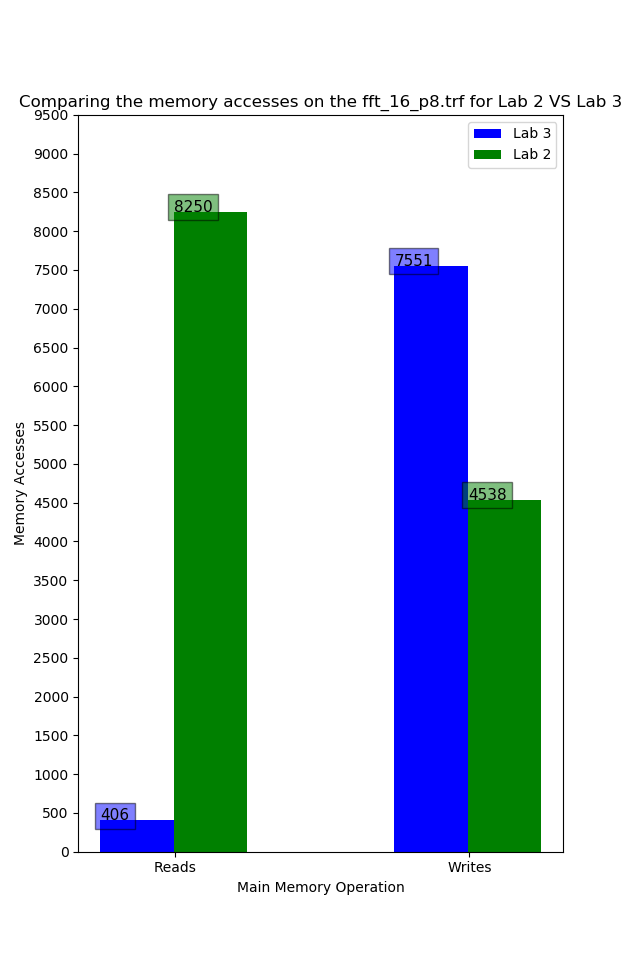
\includegraphics[scale=0.7]{lab2v3.png}
\end{figure}




\end{document}
